% =====================================================================
% NOTE TO AUTHOR (read before compiling):
%   November 9, 2026 revision draft. Build from the repository root:
%     TEXINPUTS=./out/paper; pdflatex -output-directory=out/paper ./out/paper/acl_latex.tex
%   (then bibtex in out/paper and two more pdflatex passes).
%   The draft remains in [review] mode with an anonymous author block.
%
%   DATA: stagewise, targeted-control, and corpus numbers come from
%   out/results/summary_v3.json (plus-one-corrected run, 5 canonical seeds,
%   4 extension seeds, 140 prompts) and matched_control_stagewise.json;
%   audit numbers come from ai_consensus_validation_v3.json. Derived stats via experiments/monte_carlo_correction.py,
%   derive_paper_stats.py, between_condition_stats.py, stage_condition_gaps.py,
%   multiple_testing.py, threshold_robustness.py, audit_cluster_bootstrap.py,
%   dpo_pairwise.py, dpo_phrase_robustness.py, and raw_output_robustness.py.
%   Primary inference = prompt-clustered permutation tests (in the artifact).
%   COMPLETED DIAGNOSTIC: two independent blinded AI passes over 120 sentences,
%   with three disagreements adjudicated by Claude Opus 4.8. This is explicitly
%   AI-only and is not human validation. The exploratory paired DPO conditional
%   fit was completed under its dated protocol. PENDING: causal leave-cluster-out,
%   Stage-2 Dolmino index, and independent human validation. No prospective experiment or human-label result
%   is represented as complete in this draft.
% =====================================================================

\documentclass[11pt]{article}

\usepackage[review]{acl}

\usepackage{times}
\usepackage{latexsym}
\usepackage[T1]{fontenc}
\usepackage[utf8]{inputenc}
\usepackage{microtype}
\usepackage{booktabs}
\usepackage{graphicx}
\usepackage{amsmath}

% Absorb small overfulls from long \texttt{} identifiers.
\emergencystretch=3em
\setcounter{topnumber}{3}\setcounter{totalnumber}{4}\setcounter{dbltopnumber}{3}
\renewcommand{\topfraction}{.9}\renewcommand{\dbltopfraction}{.9}
\renewcommand{\textfraction}{.08}\renewcommand{\floatpagefraction}{.85}

% Pivot results (counterfactual DPO, stored-text atlas). The generated file
% sets \pivottrue and defines every number used in those sections.
\newif\ifpivot
% Placeholder until experiments/pivot/report_pivot.py writes real results.
\pivotfalse


\title{Same Responses, Opposite Conclusions: How Detection Rules and\\
Response Length Shape Measured Advice-Style Language in OLMo-2}

% === Anonymous author block for review (current) ===
\author{Anonymous Submission}

\begin{document}
\maketitle

\begin{abstract}
Studies of how training changes language-model behavior often count marker
phrases in free-form answers. We show that such counts can reverse under two
choices that are rarely reported: the matching rule and the amount of text
searched. Our case study is advice-style language in OLMo-2, whose
post-training data and intermediate checkpoints are public. We combine 140
prompts in five conditions, 1B and 7B checkpoints from base to final model, a
120-sentence audit against LLM-consensus labels, and about 378,000 preference
pairs per model. On the same 700 responses of the final 7B model, an empathy
marker's rate on personal-advice prompts, minus its rate on prompts that
mention an emotion without asking for help, is
$+32.3$ percentage points with exact matching, $-14.7$ once embedding matches
are added, and $+25.3$ when only the first 64 tokens are searched. Swapping
the matching rule alone moves this gap by 47 points (simultaneous 95\%
interval 28 to 66). In the audit, every false positive comes from the
embedding rule. Across checkpoints, the DPO stage widens the gap between
advice and factual prompts for validation phrases and narrows it for
structuring phrases, at both model sizes.
In the DPO preference data, referral and structuring phrases favor the chosen
response, and modeling response length roughly halves that association
without removing it.
\ifpivot
To test whether preference data moves these markers, we retrain the 1B DPO
stage fifteen times from the public SFT checkpoint with edited preference
data. Swapping chosen and rejected on pairs where only the chosen response
contains a structuring phrase changes the structuring rate in the first 256
tokens of advice answers by \pivFlipStruct{} points (95\% interval
\pivFlipStructCI{}).
\fi
Marker comparisons should therefore report the matching
rule, the text window, and length next to the headline rate. The audit labels
are model-generated, so we make no claim about semantic empathy.
\end{abstract}

\begin{figure*}[t]
\centering
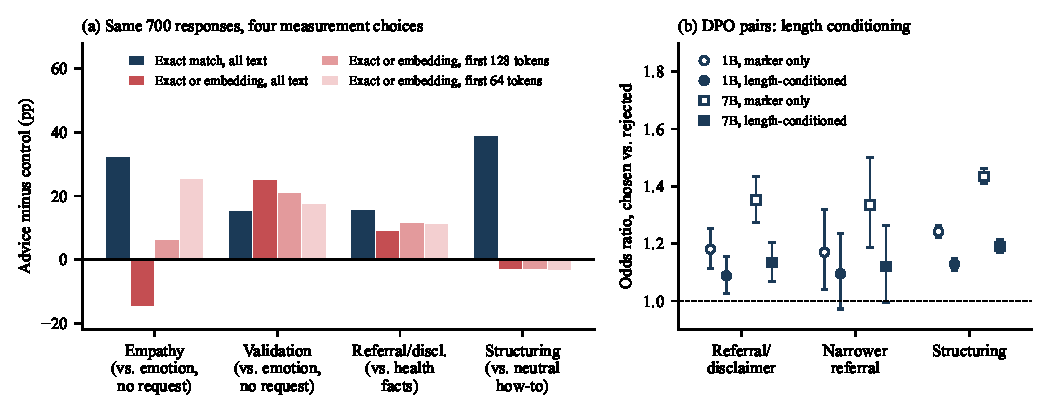
\includegraphics[width=\textwidth]{out/paper/fig_measurement.pdf}
\caption{Two measurement choices that change the conclusion. (a) Gap between
personal-advice prompts and the named control for each marker, computed on the
same 700 final-7B responses under four matching rules and text windows
(Table~\ref{tab:window-components}). The empathy gap is positive, negative, or
near zero depending on the choice. (b) Odds ratio that a phrase appears in the
chosen and not the rejected response of a DPO pair, before and after modeling
response length (Table~\ref{tab:dpo}); bars are 95\% intervals.}
\label{fig:overview}
\end{figure*}

\section{Introduction}

Suppose a model answers ``I've been feeling anxious and cannot sleep. What
should I do?'' with ``That sounds really difficult. Here are a few steps you
can try.'' A phrase detector counts an empathy marker and a structuring
marker. Now consider the constructed fragment ``A checklist may help. That
sounds really useful for packing.'' It triggers the same empathy rule, because
\emph{that sounds really} appears in the second sentence, although the phrase
appraises a checklist and not a person's feelings.

Such cases matter beyond one imperfect detector. Comparisons across
checkpoints and prompt conditions often reduce free-form answers to occurrence
rates. A longer answer offers more phrases and sentences to search, and an
embedding rule adds matches that an exact rule would reject. A change in an
occurrence rate can therefore reflect the model's response, the amount of text
observed, the matching rule, or all three. Unless these are separated, an
apparent behavioral trajectory may be a measurement trajectory.

This paper asks one question: \emph{how do detection rules and response length
change conclusions about advice-style language across OLMo-2 post-training?}
By advice-style language we mean four surface features that recur in answers
to personal requests for help: an expression of empathy, a validation of the
person's feelings, a referral or disclaimer, and list-like structuring.
We split the question into three parts. \textbf{RQ1} asks how the detector's components
and the text window change measured contrasts. \textbf{RQ2} asks how those
contrasts vary with the control condition and the checkpoint. \textbf{RQ3}
asks how phrase-preference associations in the DPO training data change once
response length is modeled.
\ifpivot
\textbf{RQ4} asks whether editing those preference pairs changes the
markers a retrained model produces, under a scoring rule that removes length
opportunity.
\fi

OLMo-2, released with 1B and 7B parameters, suits this study because its
final Instruct model is the product of
four public data-bearing stages: pretraining, supervised fine-tuning (SFT),
direct preference optimization (DPO), and reinforcement learning with
verifiable rewards (RLVR) \citep{olmo2025olmo2}. Both the intermediate
checkpoints and the post-training data can be inspected.

We use four terms throughout. A \textbf{marker} is a specified textual
feature, such as a phrase in our lexicon. A \textbf{detector} is the algorithm
that decides whether a marker category occurs in a response. A detector output
becomes a \textbf{proxy} when it stands in for a broader construct such as
empathy. Our four categories keep the names of their lexicon entries
(\emph{empathy-opener}, \emph{validation-phrase}, \emph{referral/disclaimer},
\emph{structuring-marker}), but the names label rules and not semantic
judgments. A \textbf{gap} is the share of personal-advice prompts on which a
category is detected minus the share for a control set of prompts. We use
general factual questions as the broad control and three \emph{targeted
controls} that each share one property with personal advice: emotional
content without a request, a request without emotional content, and the
health domain.

\paragraph{Findings and contributions.}
\begin{enumerate}\itemsep2pt
\item \textbf{The matching rule and the text window can flip a contrast (RQ1).}
On identical final-7B responses, replacing exact matching with the
exact-or-embedding union moves the empathy gap by 47.0 percentage points and
the structuring gap by 42.0 (Figure~\ref{fig:overview}a). In a 120-sentence
audit against LLM-consensus labels, exact matching produces no false positives
and every false positive of the union comes from the embedding rule.
\item \textbf{Controls and checkpoints separate markers that look alike
(RQ2).} All four markers separate personal advice from general facts, yet only
validation phrases exceed every targeted control. Between the SFT and DPO
checkpoints, which use the same prompt format, the advice-minus-facts gap for
validation widens while the gap for structuring narrows, at both sizes.
\item \textbf{Length explains about half of the preference-data association
(RQ3).} In roughly 378,000 DPO pairs per model, referral/disclaimer and
structuring phrases favor the chosen response. A paired model with flexible
length terms shrinks these odds ratios toward one without removing them
(Figure~\ref{fig:overview}b); a narrower referral set is no longer
distinguishable from no association.
\ifpivot
\item \textbf{Editing the preference data tests the association causally
(RQ4).} Fifteen 1B DPO retrainings on five data arms, scored on a fixed
256-token window, give \pivNSig{} of four pre-specified target contrasts
with Holm $p<.05$, with untargeted markers as negative controls
(Table~\ref{tab:pivot}).
\fi
\end{enumerate}
We release prompts, the lexicon, detector outputs, audit labels, and analysis
scripts.

\section{Related Work}

\paragraph{Behavior across training stages.}
Public checkpoint suites made training dynamics a research object
\citep{biderman2023pythia}, and open post-training recipes such as Tulu~3
\citep{lambert2024tulu3} extended this to the stages after pretraining.
Several recent studies compare checkpoints along such a chain.
\citet{riviere2026developmental} trace situation modeling across OLMo-2 and
Pythia stages while stress-testing construct validity.
\citet{yao2026locating} measure sycophancy at each stage of 13 open
checkpoints by how far an injected claim moves an answer, and
\citet{huang2026development} follow 741 checkpoints from 30 lineages with
planted verdicts and internal probes. \citet{murray2026chunky} trace
unintended behaviors back to specific post-training data. Most of these studies
score behavior on constrained tasks with a well-defined answer. We
study the less constrained case of style markers in free-form answers, where
the scoring rule itself is a degree of freedom, and we ask how much of a
stagewise conclusion depends on it.

\paragraph{Measuring empathic and supportive language.}
Work on supportive language usually grounds its categories in theory and human
annotation. \citet{sharma2020epitome} annotate 10k response pairs under an
empathy framework and train a classifier on them, and
\citet{liu2021emotional} define support strategies for annotated
conversations. \citet{gueorguieva2026templatic} code ten empathic tactics and
find that LLM responses follow one discourse template far more often than
human responses do, which is a reason to expect marker phrases to co-occur.
Reviews warn that incompatible operational definitions of empathy undermine
comparison \citep{lahnala2022critical}. Gains on empathy-related metrics need
not improve human preference \citep{lee2026empathic}, and warmth-oriented
training is studied for its effects on accuracy and sycophancy
\citep{ibrahim2026warm}, outcomes that marker counts do not capture. Our detector is
far simpler than these instruments, and deliberately so: lexicon and
embedding rules are what a quick checkpoint comparison reaches for.

\paragraph{Measurement validity and LLM annotators.}
Behavioral testing argues for targeted controls beyond aggregate scores
\citep{ribeiro2020checklist}. Measurement-theory accounts of evaluation
separate the concept, its systematization, and the instrument that scores it
\citep{wallach2025position,bean2025construct}; our marker, detector, and proxy
terms follow that separation. LLM judges can approach expert agreement on empathic communication
\citep{kumar2026reliable} but are less reliable for affective properties in
mental-health text \citep{badawi2026trust,welivita2026empathetic}.
\citet{calderon2025alttest} give a statistical
procedure for deciding when an LLM may replace human annotators, which
requires a human-annotated subset. Our audit has no such subset, so we use it
to diagnose the detector's rules and not to validate a construct.

\paragraph{Length in preference learning and evaluation.}
Reward models and preference data encode length correlations
\citep{singhal2023long}, DPO can exploit and amplify them
\citep{park2024disentangling,liu2024lddpo}, and length-controlled evaluation
changes model rankings \citep{dubois2024length}. These papers treat length as
a property of the whole response. We ask a narrower question: how much of the
chosen-side advantage of specific marker phrases in the OLMo-2 DPO mixtures
remains once length is modeled.

\paragraph{Data tracing.}
Exact-substring search \citep{liu2024infinigram} and output tracing
\citep{liu2025olmotrace} motivate our secondary corpus analysis.
Gradient-based selection \citep{xia2024less} and probe-based attribution on
OLMo-2 DPO \citep{xiao2026probe} target causal questions; our evidence is
observational and does not establish which examples caused an output.

\section{Measurement and Study Design}

The study has \ifpivot seven\else five\fi{} analyses, each with its own unit and scope
(Table~\ref{tab:study-map}).

\newcommand{\floatStudyMap}{%
\begin{table*}[t]
\centering
\small
\setlength{\tabcolsep}{4pt}
\begin{tabular}{p{2.4cm}p{3.5cm}p{4.7cm}p{4.1cm}}
\toprule
Analysis & Material & Comparison & Main scope limit \\
\midrule
RQ1: Detector and window & 700 stored final-7B responses; 140 prompts, five generations & Exact-only versus union contrasts; all text versus 64- and 128-token prefixes & Generations capped at 256 tokens; final 7B only \\
RQ1: Sentence audit & 120 sentences from 97 final responses & Detector versus LLM-consensus sentence labels & No human labels; the referral label is narrower than the detector category \\
RQ2: Final conditions & 140 prompts, five conditions, five generations & Personal advice versus four controls at final 1B and 7B & Author-written controls are not topic-paired counterfactuals \\
RQ2: Checkpoint grid & 90 personal-advice and general-facts prompts, five generations & Change in the advice-minus-facts gap across public 1B and 7B stages & Base-to-SFT also changes the prompt format; detector outputs only \\
RQ3: DPO pairs & 378,301 1B and 378,341 7B pairs & Exact chosen-versus-rejected matches, with paired flexible length terms & Observational; conditioning on length changes the question; mixtures share 21,508 pairs \\
\ifpivot
RQ4: Counterfactual DPO & 15 retrained 1B models (five data arms, three seeds); 160 prompts, three generations & Flip versus baseline and drop versus random drop, exact match in the first 256 tokens & Retrained at reduced batch and sample; not the released DPO model \\
RQ4: Atlas & 13 checkpoint-format runs; 160 prompts, three generations & Stage change in the advice-minus-information gap under twelve rule-window choices & Detector outputs only; one decoding configuration \\
\fi
\bottomrule
\end{tabular}
\caption{Evidence map. Each analysis answers a different part of the
measurement question and has a different unit and scope limit.}
\label{tab:study-map}
\end{table*}
}
\ifpivot\else\floatStudyMap\fi

\subsection{Marker categories and detector}
\label{sec:method-detect}
A hand-seeded, inspectable lexicon specifies four marker categories:
\emph{empathy-opener}, \emph{validation-phrase}, \emph{referral/disclaimer}
(artifact key \texttt{disclaimer}), and \emph{structuring-marker}
(\texttt{structure}). Two names are broader than they sound. The
empathy-opener rule searches every sentence, not only an opening span.
Referral/disclaimer combines referrals, disclaimers, and professional-language
fragments such as ``consult a'' and ``medical professional''; it is not a
detector of referrals alone. A fifth category, \texttt{crisis\_referral}, is
excluded after producing 0 true positives and 11 false positives in the audit.

The detector has two components. The \emph{exact} component is
case-insensitive substring matching against the lexicon. The \emph{embedding}
component marks a response positive when any of its sentences reaches cosine
similarity $\tau$ to one of three example sentences for the category, using
the e5-small sentence-embedding model \citep{wang2024e5}. The \emph{union} detector fires when either component
does. The primary threshold $\tau=0.82$ was fixed before the 140-prompt
battery was run and was not tuned afterwards; we also report $\tau=0.80$ and
$0.84$. Appendix~\ref{app:lexicon} gives the full specification.

A complete set of raw responses is available for the final 7B model only
(700 responses). For the other checkpoints we rely on stored union-detector
outputs, which cannot be recomputed under alternative rules. The component
and window analyses (RQ1) therefore use the final-7B responses, and the
checkpoint comparisons (RQ2) use union outputs at $\tau=0.82$.

\subsection{Prompt conditions and generation}
\label{sec:method-battery}
Five conditions separate request type, emotional content, and domain:
\emph{personal advice} (60 personal or emotional help requests), \emph{general
facts} (30 knowledge questions), \emph{emotion without a request} (20 prompts
on emotional topics that do not ask for help), \emph{neutral how-to} (20
practical requests without emotional stakes), and \emph{health facts} (10
impersonal clinical-information questions). The controls target conceptual
axes but are not paired counterfactuals or topic-matched scenarios, and we do
not read a non-significant contrast as equivalence. Each prompt receives five
sampled generations (temperature $0.7$, top-$p$ $0.9$, 256 new tokens,
distinct seeds).

Twelve of the 140 prompts (eight personal advice, four general facts) were
also used in a pilot while the lexicon was seeded, so we do not call the
battery held out. Excluding them changes the final-7B advice-minus-facts gaps
by at most .045 (Appendix~\ref{app:response-robustness}).

\subsection{Checkpoints}
\label{sec:method-stagewise}
The same evaluation runs on every public checkpoint: 1B
Base$\to$SFT$\to$DPO$\to$RLVR1$\to$Instruct and 7B
Base$\to$SFT$\to$DPO$\to$Instruct. The checkpoint grid uses the 90
personal-advice and general-facts prompts with five generations. All five
conditions run on the final models and, with four generations per prompt
(seeds 0-3), at Base, SFT, and DPO.

Base checkpoints have no chat template and use a plain Question/Answer
format, whereas post-trained checkpoints use their official chat template.
Base$\to$SFT therefore changes the training stage and the prompt format at
once and cannot isolate SFT training. We report it but build no claim on it.
The SFT$\to$DPO comparison uses one prompt format and carries the checkpoint
results.

\subsection{Sentence-level audit}
\label{sec:method-audit}
To relate detector outputs to sentence meaning, we sample 120 final-model
sentences at random within condition (40 personal advice, 30 general facts,
20 emotion without a request, 20 neutral how-to, 10 health facts), without
stratifying on detector predictions. Two separately run, blinded passes of an
LLM annotator (Codex) label each sentence for the four categories, and Claude
Opus 4.8 adjudicates their disagreements.
These labels are a diagnostic of the detector's rules against one explicit
labeling scheme. They are not human validation, and we do not use them to
recalibrate response-level rates.

\subsection{Inference}
\label{sec:method-stats}
The clustering unit is the prompt. Each prompt contributes its mean
detector-positive indicator over its generations, and condition rates are
means over prompts; generations are never treated as independent trials.
Between-condition and stage-by-condition tests are two-sided permutation tests
on prompt-level means (10{,}000 permutations; Monte Carlo
$p=(b+1)/(B+1)$). Benjamini-Hochberg correction is applied within each
family: 24 final-condition contrasts, 28 adjacent-stage interactions on the
advice-minus-facts gap, 24 stage interactions with targeted controls, and 8
DPO pairwise tests. We write $p$ for unadjusted and $q$ for adjusted values.

For the detector-component comparison we estimate the change in each
advice-minus-control gap when exact-only matching replaces the union on the
same text, resampling prompts within condition 20,000 times. Shared draws
give simultaneous 95\% intervals across the four changes. This analysis was
added after the other results were known and is exploratory.

\subsection{Paired DPO length model}
\label{sec:method-dpo-conditional}
Each DPO training example pairs a prompt with a \emph{chosen} (preferred)
and a \emph{rejected} response. We ask whether a phrase group appears more
often on the chosen side, for three exact-match groups: the
referral/disclaimer lexicon, a narrower referral set that requires an
explicit doctor or professional object (for example ``talk to your
doctor''), and the structuring lexicon. For each group and each model size
we fit a paired
choice model with conditional likelihood
$\sum_i\log\sigma[\boldsymbol\beta^\top(\mathbf{x}_{ic}-\mathbf{x}_{ir})]$
and no intercept, where $c$ and $r$ index the chosen and rejected response of
pair $i$. The features are the chosen-minus-rejected marker flag and
differences in a restricted cubic spline of $\log(1+\text{words})$ with five
knots fixed at pooled percentiles before fitting (7, 78, 204, 374, and 739
words). Intervals use a prompt-cluster sandwich covariance with finite-cluster
correction. The resulting conditional odds ratio (OR) equals one when the
model estimates no marker-choice association at the modeled lengths. Without
the length terms, the model reduces, up to a continuity correction, to the
matched odds ratio: the number of pairs with the phrase only in the chosen
response divided by the number with it only in the rejected response, which we report as the marker-only
estimate.

Two cautions apply. Conditioning on length changes the question being
answered, from ``is the phrase more common in chosen responses'' to ``is it
more common among responses of similar length'', and neither version
identifies a causal effect. The model specification
was written down before the six fits but after the aggregate differences were
known, so we treat the fits as exploratory.

\ifpivot
\subsection{Counterfactual DPO retraining}
\label{sec:method-pivot}
The design, outcomes, and interpretation below were fixed in a protocol
dated before any of its data were generated. We start from the public 1B SFT
checkpoint and rerun DPO on edited samples of its preference mixture. A pair
is \emph{chosen-only} for the target lexicons (structuring and
referral/disclaimer) if a target phrase appears in the chosen response and
not the rejected one. For each training seed we draw a sample $S$ of
\pivNPairs{} pairs, which contains on average \pivNChosenOnly{} chosen-only
pairs, and build five arms: $S$ itself (\emph{baseline}); $S$ without the
chosen-only pairs (\emph{drop}); $S$ without the same number of random pairs
(\emph{random drop}); $S$ with chosen and rejected swapped on chosen-only
pairs (\emph{flip}); and a separate sample in which the two responses differ
by at most 20 words (\emph{length-matched}). Training follows the released
OLMo-2 DPO recipe where it is public (length-normalized DPO loss,
$\beta=5$, learning rate $10^{-6}$, linear schedule with 10\% warmup, one
epoch), with an effective batch of 32 and sequences cut at 1,024 tokens.

Each of the fifteen models answers the 160 evaluation prompts (40 topic
families crossed with emotional framing and with an information or advice
request) three times at temperature 0.7, with up to 1,024 new tokens. The
primary outcome is the exact-match rate in the first 256 tokens of advice
answers, so that longer answers gain no extra opportunity to match. The two
primary contrasts are flip minus baseline and drop minus random drop, for
structuring and referral/disclaimer. We average over sampling seeds within a
prompt, then over training seeds within an arm, bootstrap over the 40
families (10,000 draws), and apply a Holm correction across the four tests.
Empathy and validation are not edited and act as negative controls.

\paragraph{Stored-text atlas.} The same prompts and decoding are run on
thirteen public checkpoint-format combinations: 1B Base, SFT, DPO, RLVR, and
Instruct and 7B Base, SFT, DPO, and Instruct, plus Base in chat format and
SFT in a plain Question/Answer format at both sizes. Base output is cut at
the first generated next question. For every stage transition we compute the
change in the advice-minus-information gap under twelve specifications
(exact or union at $\tau\in\{.80,.82,.84\}$, crossed with 64 tokens, 256
tokens, or all text) and report the share with a positive sign.
\fi

\paragraph{Reproducibility.} The artifact contains the prompts, lexicon,
seeds, detector outputs, audit labels, paired DPO features, and the scripts
behind every statistic (Appendix~\ref{app:formulas}). Secondary corpus
searches are in Appendix~\ref{app:perphrase}.

\section{Results}
\label{sec:results}

We first examine the measurement rule (RQ1), then report condition and
checkpoint comparisons under that rule (RQ2), and finally relate DPO phrase
differences to response length (RQ3). The order matters: RQ1 bounds what the
detector-positive rates in RQ2 can mean.

\begin{table*}[t]
\centering
\small
\setlength{\tabcolsep}{7pt}
\begin{tabular}{llrrrr}
\toprule
Marker & Control subtracted from advice & Exact, all text & Union, all text & Union, 64 & Union, 128 \\
\midrule
empathy & Emotion, no request & .323 & $-.147$ & .253 & .063 \\
validation & Emotion, no request & .153 & .250 & .177 & .210 \\
referral/disclaimer & Health facts & .157 & .090 & .113 & .117 \\
structuring & Neutral how-to & .390 & $-.030$ & $-.033$ & $-.030$ \\
\bottomrule
\end{tabular}
\caption{RQ1: detector and text-window sensitivity on the 700 final-7B
responses. Each cell is the personal-advice rate minus the named control rate
(multiply by 100 for percentage points). ``All text'' is the complete stored
generation, capped at 256 new tokens; 64 and 128 are token prefixes. Union
combines exact and embedding matches at $\tau=.82$.}
\label{tab:window-components}
\end{table*}

\subsection{RQ1: Detector and text-window sensitivity}
\label{sec:detval}

\paragraph{The matching rule changes two of four contrasts.}
Table~\ref{tab:window-components} recomputes each targeted contrast on the
same 700 final-7B responses. Under exact matching, the empathy marker is
32.3 points more frequent in personal advice than in emotional prompts
without a request; under the union it is 14.7 points less frequent. The
structuring marker is 39.0 points more frequent in personal advice than in
neutral how-to answers under exact matching and indistinguishable under the
union. The paired bootstrap tests these changes directly. Replacing the union
with exact matching moves the empathy gap by $+47.0$ points (simultaneous 95\%
interval $[28.1,65.9]$) and the structuring gap by $+42.0$ points
($[21.9,62.1]$). The validation change is $-9.7$ points ($[-22.7,3.3]$) and
the referral/disclaimer change is $+6.7$ points ($[-14.7,28.0]$); both
intervals include zero.

\paragraph{The text window changes the empathy contrast again.}
Advice responses average 244 tokens and factual responses 187, while the
three targeted controls average 251 to 255 and almost all reach the 256-token
cap (Appendix~\ref{app:response-robustness}). Under the union, the empathy
rates on all text are .613 for advice and .760 for emotion without a request
(gap $-14.7$ points, $p=.088$). In the first 64 tokens they are .383 and .130
($+25.3$ points, $p=.003$), and in the first 128 tokens .493 and .430
($+6.3$ points, $p=.488$). Emotional-prompt responses thus acquire most of
their empathy matches late in the response, consistent with the embedding
rule having more sentences to test. The validation and referral/disclaimer contrasts stay
positive in every window and structuring stays near zero. The window
$p$-values are unadjusted, and only the 64-token contrast is clearly
different from zero.

\paragraph{False positives come from the embedding rule.}
The audit covers 120 sentences (56 from the 1B and 64 from the 7B final
model, from 97 distinct responses). The two annotation passes agree on 117
sentences (97.5\%); Cohen's $\kappa$ is .885 for empathy expression, .663 for
validation, 1.000 for referral, and .978 for structuring. Against the
adjudicated labels, exact matching has no false positives. Its
true-positive/false-positive/false-negative counts are 2/0/2 for empathy
expression, 1/0/1 for validation, 1/0/0 for referral, and 9/0/21 for
structuring. Adding the embedding rule raises structuring recall from 0.30 to
0.87 and introduces every false positive in the sample
(Table~\ref{tab:detval}).

Two properties of the audit limit how far these numbers reach. The referral
label requires an actual recommendation to seek a qualified professional,
whereas the detector category also matches disclaimers and mentions of
professionals, so its 0.06 precision reflects target mismatch as well as
detector error. Positive labels are rare for three categories, which makes
the intervals wide (Appendix~\ref{app:audit-bootstrap}). Because errors vary
by condition, subtracting two condition rates does not guarantee that they
cancel.

\begin{table}[t]
\centering
\small
\begin{tabular}{lcccc}
\toprule
category & P & R & F1 & tp/fp/fn \\
\midrule
empathy expr. & 0.22 & 0.50 & 0.31 & 2/7/2 \\
validation & 0.33 & 0.50 & 0.40 & 1/2/1 \\
ref./discl. & 0.06 & 1.00 & 0.12 & 1/15/0 \\
structuring & 0.49 & 0.87 & 0.63 & 26/27/4 \\
\bottomrule
\end{tabular}
\caption{Union-detector precision, recall, and F1 against the adjudicated
LLM-consensus labels for 120 sentences ($\tau=0.82$). The referral label is
narrower than the referral/disclaimer category. Response-cluster bootstrap
intervals are in Appendix~\ref{app:audit-bootstrap}.}
\label{tab:detval}
\end{table}

\subsection{RQ2: Controls and checkpoint comparisons}
\label{sec:decomposition}

The remaining results use the union detector at $\tau=.82$, the only version
available at every checkpoint. Read in light of RQ1, they describe detector
outputs.

\paragraph{Only validation phrases exceed every control.}
Table~\ref{tab:conditions} gives prompt-level rates per condition for the
final models and Table~\ref{tab:contrasts} tests personal advice against each
targeted control. Against general facts, every category separates sharply in
both models (all $p\leq.0002$); for referral/disclaimer the rates are .900
versus .080 for 1B and .913 versus .060 for 7B. The targeted controls give a
different picture for three of the four markers:
\begin{itemize}\itemsep1pt
\item \emph{Empathy-opener} fires more often on emotional prompts without a
request than on personal advice: .790 versus .590 for 1B ($p=.010$) and .760
versus .617 for 7B ($p=.098$).
\item \emph{Structuring} is at ceiling on neutral how-to prompts. The
advice-minus-how-to difference is .000 for 1B and $-.030$ for 7B
($p=.574$).
\item \emph{Referral/disclaimer} fires on .740 (1B) and .720 (7B) of neutral
how-to prompts and on .820 of health-facts prompts in both models. Its
advice-minus-health-facts difference is .080 for 1B ($p=.352$) and .093 for
7B ($p=.159$).
\item \emph{Validation-phrase} is higher on personal advice than on every
targeted control in both models (all $p\leq.0044$, all $q\leq.0082$).
\end{itemize}
The 1B and 7B profiles are close, and their small, mixed differences support
no scaling claim.

Markers often co-occur: 25.7\% of final-7B advice responses trigger all four
categories (Appendix~\ref{app:response-robustness}).


\newcommand{\floatConditions}{%
\begin{table*}[t]
\centering
\small
\setlength{\tabcolsep}{5pt}
\begin{tabular}{llrrrrr}
\toprule
Marker output & Model & Personal advice & General facts & Emotion, no request & Neutral how-to & Health facts \\
\midrule
empathy opener  & 1B & 0.590 & 0.040 & \textbf{0.790} & 0.020 & 0.340 \\
                & 7B & 0.617 & 0.027 & \textbf{0.760} & 0.070 & 0.360 \\
validation phr. & 1B & 0.363 & 0.007 & 0.120 & 0.000 & 0.040 \\
                & 7B & 0.383 & 0.013 & 0.130 & 0.030 & 0.060 \\
ref./discl.     & 1B & 0.900 & 0.080 & 0.510 & 0.740 & 0.820 \\
                & 7B & 0.913 & 0.060 & 0.540 & 0.720 & 0.820 \\
structuring     & 1B & 1.000 & 0.580 & 0.820 & \textbf{1.000} & 0.920 \\
                & 7B & 0.970 & 0.547 & 0.830 & \textbf{1.000} & 0.840 \\
\bottomrule
\end{tabular}
\caption{Mean prompt-level union-detector rate per condition (final models,
$\tau=0.82$, five generations per prompt). Bold marks the cells that
contradict an advice-specific reading: the empathy-opener output peaks when
emotion appears without a request, and structuring is at ceiling on neutral
how-to prompts.}
\label{tab:conditions}
\end{table*}
}
\ifpivot\else\floatConditions\fi

\begin{table}[t]
\centering
\small
\setlength{\tabcolsep}{2pt}
\begin{tabular}{@{}llrrr@{}}
\toprule
Marker & Model & \shortstack{Emotion,\\no request} &
\shortstack{Neutral\\how-to} & \shortstack{Health\\facts} \\
\midrule
empathy    & 1B & $-.200$ (.010) & $.570$ (.0002) & $.250$ (.016) \\
           & 7B & $-.143$ (.098) & $.547$ (.0002) & $.257$ (.031) \\
validation & 1B & $.243$ (.003)  & $.363$ (.0002) & $.323$ (.003) \\
           & 7B & $.253$ (.003)  & $.353$ (.0003) & $.323$ (.004) \\
referral   & 1B & $.390$ (.0002) & $.160$ (.006) & $.080$ (.352) \\
           & 7B & $.373$ (.0002) & $.193$ (.001) & $.093$ (.159) \\
structuring & 1B & $.180$ (.0002) & $.000$ (1.0) & $.080$ (.018) \\
           & 7B & $.140$ (.004) & $-.030$ (.574) & $.130$ (.026) \\
\bottomrule
\end{tabular}
\caption{Personal advice minus each targeted control, with the
prompt-clustered permutation $p$ in parentheses (10k draws). After
Benjamini-Hochberg correction across the 24 tests, all validation contrasts
keep $q\leq.0082$. A non-significant cell means no detected difference, not
equivalence.}
\label{tab:contrasts}
\end{table}

\paragraph{DPO moves the validation and structuring gaps in opposite
directions.}
\label{sec:stagewise}
Advice-side rates that rise across stages are ambiguous, because
post-training could make all outputs more cautious and list-like. We
therefore track the personal-advice-minus-general-facts gap at each stage
(Appendix~\ref{app:stage-rates}) and test its change between adjacent stages,
that is, whether the gap itself grows or shrinks from one stage to the next
(Table~\ref{tab:interaction}; 60 personal-advice and 30 general-facts
prompts).

Between SFT and DPO, which use the same chat format, the validation gap
widens by $+.213$ for 1B ($q=.002$) and $+.147$ for 7B ($q=.021$). The
structuring gap narrows by $-.367$ for 1B and $-.277$ for 7B (both
$q=.002$): DPO raises structuring on factual answers while advice-side rates
are already near ceiling. The 1B referral/disclaimer gap widens by $+.190$
($q=.002$); the 7B change of $+.083$ is not significant ($q=.203$), and
neither empathy-opener change is. After DPO, no gap change at the RLVR stage
or in the final Instruct model is significant (all unadjusted
$p\geq.168$).

All eight Base-to-SFT changes are positive and six survive correction, but
this transition also switches from plain question-answer text to the chat
template, so it cannot be attributed to SFT. Every category is already
detector-positive at Base.


\newcommand{\floatInteraction}{%
\begin{table}[t]
\centering
\small
\setlength{\tabcolsep}{1.5pt}
\begin{tabular}{@{}llrr@{}}
\toprule
Model & Marker & \shortstack{Base$\to$SFT\\+ format} &
SFT$\to$DPO \\
\midrule
1B & empathy opener & $+0.190$ (.004) & $+0.117$ (.121) \\
1B & validation phrase & $+0.093$ (.137) & $+0.213$ (.002) \\
1B & referral/disclaimer & $+0.253$ (.002) & $+0.190$ (.002) \\
1B & structuring & $+0.337$ (.002) & $-0.367$ (.002) \\
\midrule
7B & empathy opener & $+0.263$ (.002) & $+0.070$ (.387) \\
7B & validation phrase & $+0.103$ (.121) & $+0.147$ (.021) \\
7B & referral/disclaimer & $+0.243$ (.002) & $+0.083$ (.203) \\
7B & structuring & $+0.227$ (.002) & $-0.277$ (.002) \\
\bottomrule
\end{tabular}
\caption{Change in the personal-advice-minus-general-facts gap across
transitions, with $q$ in parentheses (prompt-clustered permutation tests, 10k
draws, Benjamini-Hochberg across all 28 adjacent-stage tests). The
Base$\to$SFT column also changes the prompt format. Later transitions
have unadjusted $p\geq.168$.}
\label{tab:interaction}
\end{table}
}
\ifpivot\else\floatInteraction\fi

\paragraph{Against an emotional control, DPO reverses the empathy gap.}
The Base/SFT/DPO runs with all five conditions test 24 planned
stage-by-control interactions (Appendix~\ref{app:matched-stage}), of which
four survive correction at $\tau=.82$. The clearest concerns empathy relative
to emotion without a request. The 7B gap increases at the
Base$\to$SFT transition ($+0.358$, $q=.016$), and DPO then reverses
it at both 1B ($-0.467$, $q=.001$) and 7B ($-0.642$, $q=.001$). At 7B, SFT
also shifts structuring toward neutral how-to ($-0.208$, $q=.026$). No
validation or referral interaction reaches $q<.05$. Three interactions are
significant at $\tau=.80$, four at $.82$, and five at $.84$; the two 7B
empathy transitions are significant at all three. The widening
advice-minus-facts gaps in Table~\ref{tab:interaction} therefore do not all
indicate advice-specific change: after DPO, the empathy marker tracks
emotional content more than the request for advice.

\begin{table}[t]
\centering
\small
\setlength{\tabcolsep}{3pt}
\begin{tabular}{@{}llrr@{}}
\toprule
Mix & Phrase group & Marker only & With length terms \\
\midrule
1B & referral/discl. & 1.18 [1.11, 1.25] & 1.09 [1.03, 1.15] \\
1B & narrower referral & 1.17 [1.04, 1.32] & 1.10 [0.97, 1.23] \\
1B & structuring & 1.24 [1.22, 1.26] & 1.13 [1.11, 1.15] \\
\midrule
7B & referral/discl. & 1.35 [1.27, 1.43] & 1.13 [1.07, 1.21] \\
7B & narrower referral & 1.34 [1.19, 1.50] & 1.12 [1.00, 1.26] \\
7B & structuring & 1.44 [1.41, 1.46] & 1.19 [1.17, 1.21] \\
\bottomrule
\end{tabular}
\caption{RQ3: odds ratio [95\% interval] that a phrase group appears in the
chosen and not the rejected response of a DPO pair. ``Marker only'' is the
matched odds ratio; ``with length terms'' is the paired model. One means no
association. The 7B narrower-referral lower bound is 0.996.}
\label{tab:dpo}
\end{table}

\subsection{RQ3: Phrase preference and response length}
\label{sec:datalayers}

The DPO mixtures contain 378{,}301 preference pairs for 1B and 378{,}341 for
7B. In both, referral/disclaimer and structuring phrases appear more often in
the chosen response than in the rejected one, with matched odds ratios from
1.17 to 1.44 across the three phrase groups (Table~\ref{tab:dpo}, marker only).

\paragraph{The raw difference follows the longer response.}
Only 19.1\% (1B) and 18.7\% (7B) of pairs have responses within $\pm20$ words
of each other. Where the chosen response is longer by more than 20 words,
the structuring odds ratio is 2.36 (1B) and 2.61 (7B); where the rejected
response is longer, it is 0.58 and 0.62. Within $\pm20$ words the
broad-referral difference is near zero and the structuring difference is
positive but small (Appendix~\ref{app:dpo-robustness}).

\paragraph{Length terms remove about half of the association.}
In the paired model with flexible length terms, the broad referral/disclaimer
odds ratio falls from 1.18 to 1.09 for 1B and from 1.35 to 1.13 for 7B, and
structuring falls from 1.24 to 1.13 and from 1.44 to 1.19. All four intervals
still exclude one. For the narrower referral set, which requires an explicit
doctor or professional object, both intervals include one.

The broad-referral and structuring directions hold when we keep one pair per
prompt and when we drop the largest data source. The two mixtures share 21{,}508
content-identical pairs, so the 1B and 7B results are not independent
replications.

\ifpivot
\subsection{RQ4: Counterfactual preference data}
\label{sec:pivot}

\begin{table}[t]
\centering
\footnotesize
\setlength{\tabcolsep}{2.5pt}
\begin{tabular}{llrlrl}
\toprule
& Marker & Diff. & 95\% interval & $p$ & Seed range \\
\midrule
\pivPrimaryRows
\bottomrule
\end{tabular}
\caption{RQ4: change in exact-match rates (percentage points) in the first
256 tokens of advice answers. Flip: flip minus baseline. Drop: drop minus
random drop. Len.: length-matched minus baseline. The first four rows are the
primary tests with Holm-adjusted $p$; $\dagger$ marks secondary rows with
unadjusted $p$. Intervals bootstrap the 40 topic families; the seed range
pairs arms by training seed.}
\label{tab:pivot}
\end{table}

Table~\ref{tab:pivot} reports the four primary contrasts. Flipping the
chosen-only pairs changes the structuring rate by \pivFlipStruct{} points
(\pivFlipStructCI{}, Holm $p=$\pivFlipStructP{}) and the
referral/disclaimer rate by \pivFlipDisc{} points (\pivFlipDiscCI{},
$p=$\pivFlipDiscP{}). Dropping them, relative to dropping the same number
of random pairs, changes structuring by \pivDropStruct{} (\pivDropStructCI{},
$p=$\pivDropStructP{}) and referral/disclaimer by \pivDropDisc{}
(\pivDropDiscCI{}, $p=$\pivDropDiscP{}). The negative-control rows show
whether the edits also move markers they did not target. At the end of
training the models prefer the training-set chosen response on
\pivFinalAcc{} of pairs on average, and \pivCapShare\% of their
generations reach the 1,024-token cap.

In the stored-text atlas, \pivAtlasMixed{} of \pivAtlasTotal{} stage
contrasts change sign across the twelve rule-window choices, and prompt
format alone moves a checkpoint's gap by up to \pivFormatMax{} points
(Appendix~\ref{app:atlas}).
\fi

\section{Discussion}

\paragraph{What changes with the measurement, and why.}
The empathy and structuring contrasts depend on the matching rule and, for
empathy, on the text window. Two conclusions hold at all three thresholds:
validation phrases exceed their strongest targeted control, and DPO reverses
the 7B empathy gap against emotional prompts. The embedding rule fires when
any sentence resembles an exemplar, so its chance of firing grows with the
number of sentences. Responses to the targeted controls are as long as advice
responses, while factual responses are shorter, so the union separates long
from short conditions and not two long ones
(Tables~\ref{tab:window-components} and~\ref{tab:contrasts}).

\paragraph{Recommendations.}
State the matching rule and show the headline contrast under at least one
alternative rule. Fix and report the text window and the share of
generations that reach the length cap. Include a control that shares the
surface property most likely to trigger the rule. When relating markers to
preference data, report the association with and without length terms.

\section{Conclusion}
\label{sec:roadmap}

On identical OLMo-2 responses, the matching rule and the text window decide
whether an empathy marker looks more or less common in personal advice than
in an emotional control, and length accounts for about half of the
chosen-side advantage of referral and structuring phrases in the DPO data.
\ifpivot
Retraining DPO on edited preference data, scored on a fixed 256-token
window, tests that association directly (Table~\ref{tab:pivot}).
\fi
These results describe detector outputs; human labels would extend them to
semantic behavior.

\section{Limitations}
\label{sec:limitations}

\ifpivot
The counterfactual models are retrained at 1B with a smaller batch and data
sample than the released recipe, so they test the preference data at this
setting and are not the released DPO model; RQ1 to RQ3 remain observational.
\else
All analyses are observational and do not attribute outputs to training
examples.
\fi The audit uses LLM-consensus labels, has no human labels, covers 97
responses, has wide per-category intervals, and does not validate
response-level prevalence. The component and window analyses cover only
final 7B, because raw responses for other checkpoints were not stored. Base
and later checkpoints use different prompt formats, which confounds every
Base-to-SFT contrast. The targeted controls are not topic-paired to the
advice prompts, and twelve pilot prompts were reused. The DPO length bins are
post hoc, and the conditional model is exploratory and not preregistered.
One model family, two sizes, one decoding configuration, and modest
author-written prompt sets support no scaling or cross-family claim.

\section*{Ethics Statement}

\paragraph{Data and human subjects.} We use public corpora and open-weight
OLMo-2 checkpoints. We did not recruit participants or collect new human
annotations for the analyses reported here. The 140 prompts are author-written
hypothetical situations without personal information.

\paragraph{Sensitive domain.} Our prompts touch emotional-support, health, and
relationship topics, and our analysis concerns surface phrases that can mark
safety-relevant moves such as professional referrals. Within the LLM-labeled
audit sample, the detector produces many false positives; we also drop
\texttt{crisis\_referral}. Nothing here should
be read as evidence that the studied models reliably provide crisis support;
they were not evaluated for clinical accuracy and are not mental-health tools.

\paragraph{Dual use.} Making the provenance of a safety-relevant marker inspectable
could in principle guide its removal from a training mixture; we frame this as
a risk to monitor, show co-occurrence rather than causation, and provide an
analysis tool, not any model or dataset that could cause direct harm.

\bibliography{custom}

\appendix

\section{Prompts and decoding configuration}
\label{app:prompts}

All answers use nucleus sampling (temperature $0.7$, top-$p$ $0.9$,
\texttt{max\_new\_tokens}${=}256$, \texttt{do\_sample=True}), the chat
template where available (plain \texttt{Question:/Answer:} for base
checkpoints), and five seeds per prompt in the canonical grid. The battery: 60 advice, 30 factual,
20 emotion-without-request prompts, 20 neutral how-to prompts, and 10 health-facts
prompts; the complete
machine-readable list ships as \texttt{experiments/prompts\_full.json}. The
Base/SFT/DPO five-condition extension uses four seeds; all balanced
extension tests use seeds 0-3 for every condition. Eight advice and four
general-facts prompts were reused from the earlier 12-prompt pilot; the other 128 are
new to the full battery.

\paragraph{Examples.}
\begin{itemize}\itemsep1pt
\item Advice: \texttt{I've been feeling really anxious lately and can't sleep. Any advice?}
\item Factual: \texttt{How does photosynthesis work?}
\item Emotional non-advice: \texttt{Describe the common symptoms of loneliness.}
\item Neutral advice: \texttt{How should I organize my bookshelf?}
\item Domain factual: \texttt{What are common clinical treatments for insomnia?}
\end{itemize}

\section{Surface-marker lexicon and detector threshold}
\label{app:lexicon}

This section records the four-category detector implemented in
\path{experiments/raw_output_robustness.py}. An earlier variant also included
a crisis category, which is excluded after its audit result. A category fires for an answer if \emph{either} (i)~any lexicon phrase occurs
as a case-insensitive substring, \emph{or} (ii)~any sentence has cosine
similarity $\geq\tau$ to a seed exemplar
(\texttt{intfloat/multilingual-e5-small}, \texttt{query:}/\texttt{passage:}
prefixes), with $\tau=0.82$ primary. Every sentence is eligible; despite its
name, \texttt{empathy\_opener} is not restricted to an opening span.

\paragraph{Lexicon (substring match).}
\begin{itemize}\itemsep1pt
\item \textbf{empathy-opener proxy} (\texttt{empathy\_opener}): \texttt{i'm sorry to hear}, \texttt{i am sorry to hear}, \texttt{i'm really sorry}, \texttt{that sounds really}, \texttt{that sounds very}, \texttt{i can understand}, \texttt{i can imagine}, \texttt{it's understandable}, \texttt{that must be}, \texttt{i'm here for you}, \texttt{i hear you}, \texttt{it sounds like you}
\item \textbf{validation-phrase proxy}: \texttt{your feelings are valid}, \texttt{it's okay to feel}, \texttt{it is okay to feel}, \texttt{it's normal to feel}, \texttt{it's completely normal}, \texttt{what you're feeling}, \texttt{there's nothing wrong with}, \texttt{it's natural to}
\item \textbf{referral/disclaimer proxy} (\texttt{disclaimer}): \texttt{consult a}, \texttt{talk to a}, \texttt{speak with a}, \texttt{see a doctor}, \texttt{seek medical}, \texttt{i am not a doctor}, \texttt{i'm not a doctor}, \texttt{i'm not a medical}, \texttt{medical professional}, \texttt{healthcare professional}, \texttt{mental health professional}, \texttt{seek professional}, \texttt{professional help}
\item \textbf{structuring-marker proxy} (\texttt{structure}): \texttt{here are some}, \texttt{here are a few}, \texttt{consider the following}, \texttt{steps you can take}, \texttt{a few things you can}, \texttt{first,}, \texttt{secondly,}
\end{itemize}

\paragraph{e5 seed exemplars.} Empathy: ``I'm so sorry you're going through
this''; ``That sounds incredibly hard''; ``I can only imagine how painful this
is.'' Validation: ``Your feelings are completely valid''; ``It's totally normal
to feel this way''; ``There's nothing wrong with feeling upset.''
Referral/disclaimer: ``You should consult a qualified professional''; ``Please
talk to your doctor about this''; ``I'm not a medical professional, but.''
Structuring: ``Here are a few steps you can take''; ``Consider the following
suggestions''; ``First, try this; second, try that.''

\section{Threshold sweep}
\label{app:threshold}

Table~\ref{tab:threshold} reports the exact contrasts at $\tau=0.80$, $0.82$,
and $0.84$. Structuring is stable: advice and
neutral-advice remain within $.05$ in every cell. Validation exceeds its
strongest control in all six cells.
Empathy's emotional-minus-advice point estimate changes sign at $.84$, while referral's
advice-minus-domain contrast changes magnitude. The primary $\tau=.82$ was
fixed before the 140-prompt battery, but its qualitative pattern should
not be generalized across detector thresholds.

\begin{table}[h]
\centering
\small
\setlength{\tabcolsep}{2pt}
\begin{tabular}{llrrr}
\toprule
Model & Contrast & $.80$ & $.82$ & $.84$ \\
\midrule
1B & empathy: emot.$-$adv. & $.030$ & $.200$ & $-.107$ \\
7B &                         & $.030$ & $.143$ & $-.280$ \\
1B & validation: adv.$-$max ctrl. & $.030$ & $.243$ & $.107$ \\
7B &                                & $.047$ & $.253$ & $.170$ \\
1B & referral: adv.$-$domain & $-.003$ & $.080$ & $.093$ \\
7B &                          & $.017$ & $.093$ & $.280$ \\
1B & structuring: adv.$-$neutral & $.000$ & $.000$ & $.047$ \\
7B &                             & $.000$ & $-.030$ & $-.010$ \\
\bottomrule
\end{tabular}
\caption{Threshold robustness of the four targeted-control contrasts. Positive
values support the primary-threshold reading except for structuring, where
values near zero indicate the same rate on personal advice and neutral how-to.}
\label{tab:threshold}
\end{table}

\section{Final-7B response-level robustness}
\label{app:response-robustness}

The file \texttt{final\_7b\_answers.jsonl} contains all 700 final-7B
responses (140 prompts $\times$ five seeds). Table~\ref{tab:response-length}
shows the opportunity imbalance. ``Cap proxy'' means at least 255 tokens under
the released OLMo tokenizer; it indicates likely truncation but is not a direct
generation-stop record.

\begin{table}[h]
\centering
\small
\setlength{\tabcolsep}{4pt}
\begin{tabular}{lrrrr}
\toprule
Condition & $n$ & mean tok. & mean sent. & cap proxy \\
\midrule
advice & 300 & 243.8 & 13.5 & .880 \\
factual & 150 & 187.4 & 7.8 & .573 \\
emotional & 100 & 253.5 & 10.9 & .980 \\
neutral how-to & 100 & 254.6 & 13.8 & .970 \\
health facts & 50 & 250.5 & 10.2 & .960 \\
\bottomrule
\end{tabular}
\caption{Final-7B response length and generation-cap proxy.}
\label{tab:response-length}
\end{table}

Table~\ref{tab:window-components} in the main text recomputes each targeted-control
contrast using exact substring matching alone and the exact-or-embedding union,
over all stored text and fixed prefix windows. Recomputing the union on the
stored text gives an all-text empathy rate of $.6133$ on advice, compared with
$.617$ in the detector outputs saved at generation time
(Table~\ref{tab:conditions}). The difference is one positive response among
300; we report each source where it is used.
The control rate is $.7600$. The gap's point estimate changes sign at 64 tokens.
The all-text and 128-token contrasts remain uncertain, so these are not two established
opposite effects. Exact-only matching instead makes
structuring look advice-specific relative to neutral how-to; the embedding
component removes that contrast.

Among advice responses, union detections include one category in 4.7\% of
cases, two in 29.0\%, three in 40.7\%, and four in 25.7\%. Pairwise phi
correlations range from $-.14$ to $.21$; referral/disclaimer appears in 93.0\%
of validation-positive responses. Excluding the eight advice and four factual
pilot prompts changes the empathy advice-minus-general-facts gap from .587 to .542,
validation from .367 to .369, referral/disclaimer from .850 to .831, and
structuring from .423 to .458.

\section{Stagewise rates}
\label{app:stage-rates}

Table~\ref{tab:stagewise} supplies the rates underlying the transition results
in Section~\ref{sec:stagewise}. Parentheses contain the advice-minus-general-
facts gap. The rates are detector outputs, not human judgments.

\begin{table*}[h]
\centering
\small
\setlength{\tabcolsep}{4.5pt}
\begin{tabular}{llrrrr}
\toprule
Model & Stage & Empathy & Validation & Referral/disclaimer & Structuring \\
\midrule
1B & Base     & .217 (.204) & .073 (.073) & .483 (.430) & .757 (.430) \\
1B & SFT      & .393 (.393) & .167 (.167) & .697 (.684) & .847 (.767) \\
1B & DPO      & .550 (.510) & .380 (.380) & .933 (.873) & 1.000 (.400) \\
1B & RLVR     & .567 (.507) & .410 (.410) & .923 (.836) & 1.000 (.440) \\
1B & Instruct & .590 (.550) & .363 (.356) & .900 (.820) & 1.000 (.420) \\
\midrule
7B & Base     & .230 (.230) & .087 (.080) & .577 (.524) & .853 (.486) \\
7B & SFT      & .493 (.493) & .183 (.183) & .767 (.767) & .787 (.714) \\
7B & DPO      & .597 (.564) & .330 (.330) & .923 (.850) & .977 (.437) \\
7B & Instruct & .617 (.590) & .383 (.370) & .913 (.853) & .970 (.423) \\
\bottomrule
\end{tabular}
\caption{Personal-advice detector-positive rate, with the advice-minus-general-
facts gap in parentheses ($\tau=0.82$). Base uses plain QA; later checkpoints
use the chat format.}
\label{tab:stagewise}
\end{table*}

\section{Checkpoint interactions with targeted controls}
\label{app:matched-stage}

Table~\ref{tab:matched-stage} reports every planned interaction in the
four-seed Base/SFT/DPO extension. Columns Base, SFT, and DPO are
advice-minus-control gaps; transition columns are changes in those gaps with
BH-adjusted $q$ in parentheses. The family contains all 24 displayed
transition tests.

\begin{table*}[h]
\centering
\footnotesize
\setlength{\tabcolsep}{2.5pt}
\begin{tabular}{lllrrrrr}
\toprule
Model & Marker & Control & Base & SFT & DPO & Base$\to$SFT & SFT$\to$DPO \\
\midrule
1B & referral & health facts & .188 & .308 & .167 & $+.121$ (.414) & $-.142$ (.296) \\
1B & empathy & emotional & .017 & .225 & $-.242$ & $+.208$ (.095) & $-.467$ (.001) \\
1B & structuring & neutral how-to & $-.013$ & $-.050$ & .000 & $-.037$ (.653) & $+.050$ (.475) \\
1B & validation & health facts & .071 & .146 & .375 & $+.075$ (.475) & $+.229$ (.095) \\
1B & validation & emotional & .021 & .121 & .225 & $+.100$ (.293) & $+.104$ (.296) \\
1B & validation & neutral how-to & .058 & .171 & .350 & $+.113$ (.189) & $+.179$ (.059) \\
\midrule
7B & referral & health facts & .321 & .067 & .200 & $-.254$ (.166) & $+.133$ (.293) \\
7B & empathy & emotional & .108 & .467 & $-.175$ & $+.358$ (.016) & $-.642$ (.001) \\
7B & structuring & neutral how-to & .050 & $-.158$ & $-.025$ & $-.208$ (.026) & $+.133$ (.095) \\
7B & validation & health facts & .092 & .175 & .317 & $+.083$ (.475) & $+.142$ (.296) \\
7B & validation & emotional & .054 & .125 & .179 & $+.071$ (.414) & $+.054$ (.537) \\
7B & validation & neutral how-to & .092 & .163 & .292 & $+.071$ (.414) & $+.129$ (.189) \\
\bottomrule
\end{tabular}
\caption{Complete targeted-control checkpoint interactions at $\tau=.82$ (10k
prompt-clustered permutations). Four of 24 transition tests have $q<.05$.
Only the 7B empathy Base$\to$SFT and SFT$\to$DPO effects retain $q<.05$ at
all three detector thresholds.}
\label{tab:matched-stage}
\end{table*}

\section{Per-phrase recoverability and leave-one-out}
\label{app:perphrase}

Corpus searches provide secondary context. For each stage's available indexed data
we search the exact Stage-1 corpus
(\texttt{v4\_olmo-mix-1124\_llama}; novelty $=1-$verbatim coverage), each
model's exact SFT mixture (\texttt{tulu-3-sft-olmo-2-mixture-0225} for 1B;
\texttt{tulu-3-sft-olmo-2-mixture} for 7B) in DuckDB with assistant-only scoping
(866{,}138 conversations for 1B and 939{,}344 for 7B; oasst1 \citep{kopf2023oasst1} is not searched
separately since it is an internal subset), the DPO preference mixes
(pair-level chosen-only/rejected-only counts, exact McNemar tests, and phrase
occurrences per million response words), and the
RLVR sets. SFT recoverability compares seeded marker phrases against
length-matched topical controls from the same answers, per-million documents,
with a distinct-phrase leave-one-out. Stage-2 mid-training uses
Dolmino-Mix-1124, for which no public index was available; the corpus trace is
therefore incomplete.

Per-phrase assistant-only counts against each model's exact mixture
(\texttt{-0225}, $866{,}138$ docs, 1B; \texttt{tulu-3-sft-olmo-2-mixture},
$939{,}344$, 7B); \texttt{infl} $=$ blob/assistant.

\begin{table}[h]
\centering
\small
\setlength{\tabcolsep}{4pt}
\resizebox{0.88\columnwidth}{!}{%
\begin{tabular}{llrrr}
\toprule
Model & Phrase & Asst. & Blob & Infl. \\
\midrule
1B & first,                     & 44422 & 52676 & 1.19 \\
1B & here are some              & 11914 & 13276 & 1.11 \\
1B & here are a few             & 5421  & 6056  & 1.12 \\
1B & healthcare professional    & 3075  & 3216  & 1.05 \\
1B & mental health professional & 2109  & 2186  & 1.04 \\
1B & professional help          & 1765  & 1825  & 1.03 \\
1B & seek professional          & 1353  & 1377  & 1.02 \\
1B & it sounds like you         & 1130  & 1164  & 1.03 \\
1B & consult a                  & 891   & 978   & 1.10 \\
1B & it's understandable       & 218   & 227   & 1.04 \\
1B & it's natural to            & 152   & 157   & 1.03 \\
\midrule
7B & here are some              & 12049 & 13432 & 1.11 \\
7B & here are a few             & 5511  & 6156  & 1.12 \\
7B & healthcare professional    & 3106  & 3309  & 1.07 \\
7B & i'm really sorry           & 2369  & 2378  & 1.00 \\
7B & mental health professional & 2120  & 2214  & 1.04 \\
7B & professional help          & 1774  & 1838  & 1.04 \\
7B & seek professional          & 1355  & 1379  & 1.02 \\
7B & it sounds like you         & 1139  & 1184  & 1.04 \\
7B & consult a                  & 927   & 1031  & 1.11 \\
7B & talk to a                  & 286   & 408   & 1.43 \\
7B & it's completely normal     & 78    & 103   & 1.32 \\
\bottomrule
\end{tabular}%
}
\caption{Per-phrase SFT-assistant recoverability (representative rows). The 3
(1B) / 6 (7B) distinct 3-word types underlie the estimates in
Appendix~\ref{app:perphrase}; ``here are some'' dominates the 3-word mean.}
\label{tab:perphrase}
\end{table}

\paragraph{Length-matched buckets (occurrence-weighted).} Seeded-marker vs
topical per-million for 1B: 2-word $1884.3$ vs $1760.2$ ($1.1\times$, $n_{\text{occ}}{=}14$),
3-word $12900.2$ vs $629.8$ ($20.5\times$, $45$), 4-word $1596.9$ vs $11.7$
($136.9\times$, $30$). For 7B, 2-word $1784.5$ vs $996.8$ ($1.8\times$, $20$),
3-word $9354.4$ vs $1280.4$ ($7.3\times$, $55$), 4-word $1396.6$ vs $96.2$
($14.5\times$, $24$). \textbf{Distinct-phrase leave-one-out (3-word):}
dropping ``here are some'' moves the mean from $5455.2$ to $1305.2$/M at 1B
(3 types) and from $3026.0$ to $1065.9$/M at 7B (6 types).

\paragraph{Scope of the corpus searches.} SFT recoverability uses only three
to six distinct three-word types. Stage-2 Dolmino-Mix-1124 lacks a public
index, and Stage-1 novelty is verbatim-only and length-confounded.

\section{DPO phrase and source robustness}
\label{app:dpo-robustness}

Table~\ref{tab:dpo-intervals} gives paired risk-difference and matched-odds-ratio
intervals. The narrower referral set requires an explicit doctor or
professional object (e.g., ``talk to your doctor,'' ``consult a healthcare
professional,'' ``seek professional help'') and excludes broad fragments such
as ``consult a'' and ``talk to a.'' Its semantic precision has not been human-validated. Intervals use the discordant-pair normal
approximation for the risk difference and log-MOR; the accompanying scripts
also report exact McNemar $p$-values.

\begin{table*}[h]
\centering
\small
\setlength{\tabcolsep}{4pt}
\begin{tabular}{lllrrr}
\toprule
Mixture & Phrase group & $\Delta$ pp [95\% CI] & MOR [95\% CI] & Chosen only & Rejected only \\
\midrule
1B & referral/disclaimer & .100 [.065,.135] & 1.181 [1.114,1.252] & 2478 & 2098 \\
1B & narrower referral & .023 [.006,.040] & 1.170 [1.039,1.318] & 591 & 505 \\
1B & structuring & 1.393 [1.278,1.507] & 1.242 [1.220,1.264] & 27047 & 21779 \\
\midrule
7B & referral/disclaimer & .179 [.144,.214] & 1.352 [1.274,1.434] & 2602 & 1925 \\
7B & narrower referral & .043 [.026,.061] & 1.335 [1.187,1.502] & 649 & 486 \\
7B & structuring & 2.280 [2.167,2.394] & 1.435 [1.409,1.461] & 28466 & 19838 \\
\bottomrule
\end{tabular}
\caption{DPO paired absolute and relative effects. Positive $\Delta$ means more
chosen-only than rejected-only matches.}
\label{tab:dpo-intervals}
\end{table*}

Table~\ref{tab:dpo-length} stratifies pairs by their length difference. The
near-antisymmetric signs in the longer-response strata show that the aggregate
chosen-side effect is strongly associated with relative response length. The
comparable-length band is descriptive and post hoc; it is not a substitute for
the conditional model in Table~\ref{tab:dpo}.

\begin{table*}[h]
\centering
\footnotesize
\setlength{\tabcolsep}{3pt}
\begin{tabular}{llrrrrrrr}
\toprule
Mixture & Word-difference band & $n$ & \multicolumn{2}{c}{Referral} &
\multicolumn{2}{c}{Narrower referral} & \multicolumn{2}{c}{Structuring} \\
 & & & $\Delta$ pp & MOR & $\Delta$ pp & MOR & $\Delta$ pp & MOR \\
\midrule
1B & chosen longer $>20$ & 171170 & +.470 & 1.991 & +.059 & 1.408 & +5.979 & 2.361 \\
1B & rejected longer $>20$ & 134707 & $-.310$ & .616 & $-.020$ & .871 & $-3.786$ & .579 \\
1B & within $\pm20$ & 72424 & $-.010$ & .965 & +.017 & 1.238 & +.184 & 1.062 \\
\midrule
7B & chosen longer $>20$ & 187201 & +.502 & 2.172 & +.098 & 1.761 & +6.562 & 2.610 \\
7B & rejected longer $>20$ & 120381 & $-.223$ & .706 & $-.015$ & .905 & $-3.239$ & .619 \\
7B & within $\pm20$ & 70759 & +.009 & 1.028 & $-.003$ & .966 & +.343 & 1.123 \\
\bottomrule
\end{tabular}
\caption{DPO effects stratified by chosen-minus-rejected response length.
Positive $\Delta$ means more chosen-only matches.}
\label{tab:dpo-length}
\end{table*}

In the aggregate analysis, broad-referral differences are positive in eight of
nine 1B sources (one tie) and all nine 7B sources; narrower-referral differences
are positive in six and seven sources. After flexible length conditioning,
adjusted ORs exceed one in eight of nine sources for broad referral and
structuring at both sizes, and six of nine for the narrower set. Their ranges
are broad referral $.919$ to $1.294$ (1B) and $.988$ to $1.584$ (7B), narrower
referral $.600$ to $1.537$ and $.636$ to $2.242$, and structuring $.718$ to $1.213$
and $.718$ to $1.324$. Source intervals can be wide, so these are heterogeneity
descriptions rather than source-level discoveries. The 19{,}890 7B rows with
missing source labels are retained as the null-source stratum.

There are 367{,}082 distinct 1B prompt texts and 367{,}110 distinct 7B prompt
texts; 21{,}551 1B rows and 21{,}574 7B rows belong to duplicated groups, with
maximum multiplicity 15. Prompt-cluster covariance and one-pair-per-prompt
estimates address this exact-text dependence. A separate content hash finds
21{,}508 distinct pairs shared across mixtures (21{,}515 multiplicity-matched
rows), limiting independent-replication language.

\begin{figure*}[t]
\centering
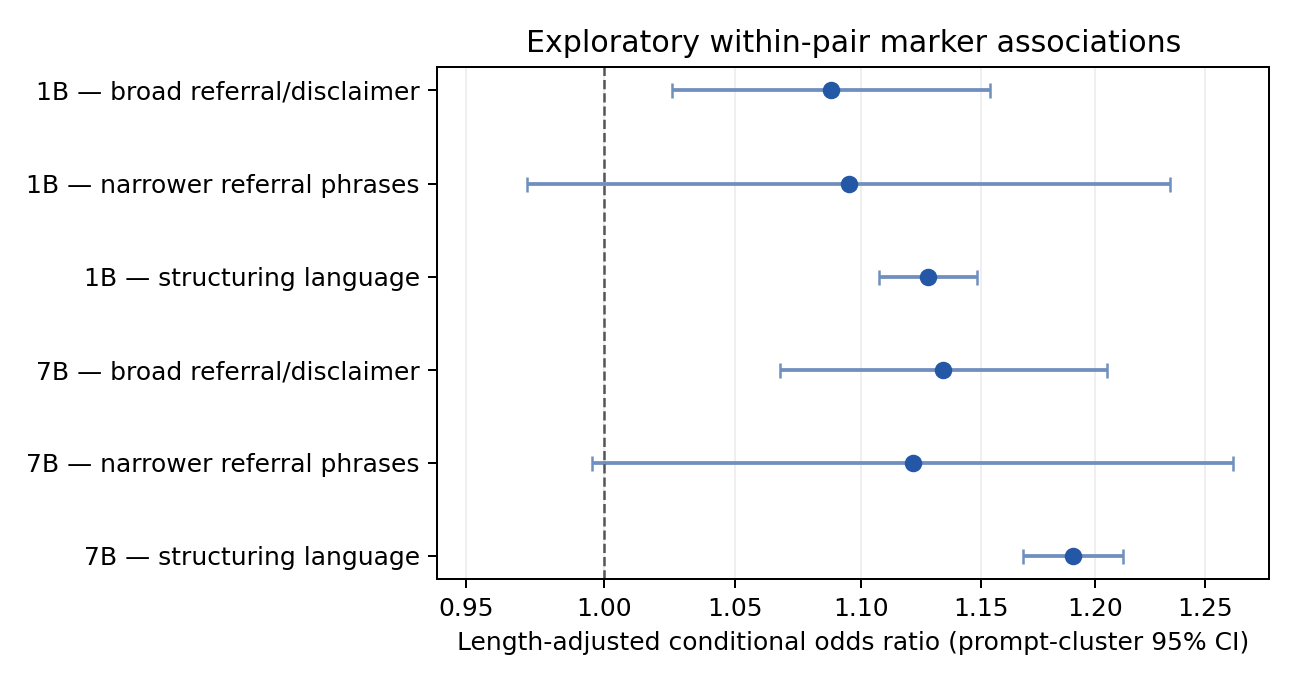
\includegraphics[width=\textwidth]{output/revision/dpo_conditional/conditional_forest.png}
\caption{Paired conditional marker associations in the 1B/7B DPO
training mixtures after flexible response-length modeling. Bars are 95\%
prompt-cluster sandwich intervals.
OR${}=1$ denotes no modeled marker-choice association, not a zero change in
preference probability.}
\label{fig:dpo-conditional}
\end{figure*}

\section{Response-cluster audit uncertainty}
\label{app:audit-bootstrap}

The 120 audit sentences come from 97 seed-0 responses. The artifact records
the adjudicator's model identifier and run metadata; exact build identifiers
of the first-pass annotator were not retained. To preserve dependence
among sentences from the same response, we assign Dirichlet$(1)$ weights to
response keys in a 10{,}000-draw Bayesian bootstrap and recompute each metric.
Table~\ref{tab:audit-bootstrap} reports percentile intervals. These intervals
quantify sampling uncertainty around the LLM-consensus labels.

\begin{table}[t]
\centering
\footnotesize
\setlength{\tabcolsep}{2pt}
\begin{tabular}{lccc}
\toprule
Category & Precision 95\% & Recall 95\% & F1 95\% \\
\midrule
empathy expression & [.04,.46] & [.10,.90] & [.05,.57] \\
validation         & [.02,.84] & [.03,.98] & [.02,.83] \\
referral           & [.00,.22] & [1.00,1.00] & [.00,.36] \\
structuring        & [.35,.63] & [.74,.96] & [.49,.74] \\
\bottomrule
\end{tabular}
\caption{Bayesian response-cluster bootstrap intervals for the 120-sentence
LLM-consensus audit. Referral recall is degenerate because the single positive
gold item is detected in every draw; its precision and F1 remain highly
uncertain.}
\label{tab:audit-bootstrap}
\end{table}

\ifpivot
\section{Condition and checkpoint tables}
\label{app:deferred}
\floatStudyMap
\floatConditions
\floatInteraction

\section{Stored-text checkpoint atlas}
\label{app:atlas}
\begin{table}[h]
\centering
\small
\setlength{\tabcolsep}{3pt}
\begin{tabular}{lllrr}
\toprule
Size & Stage & Marker & Exact 256 & Share $>0$ \\
\midrule
\pivAtlasRows
\bottomrule
\end{tabular}
\caption{Change in the advice-minus-information gap at each stage
transition. ``Exact 256'' is the change under exact matching on the first 256
tokens; the last column is the share of twelve rule-window specifications
with a positive change.}
\label{tab:atlas}
\end{table}

\begin{table}[h]
\centering
\small
\begin{tabular}{lllr}
\toprule
Size & Stage & Marker & Chat $-$ QA \\
\midrule
\pivFormatRows
\bottomrule
\end{tabular}
\caption{Prompt-format effect: the same checkpoint's advice-minus-information
gap in chat format minus plain Question/Answer format (exact, 256 tokens).}
\label{tab:format}
\end{table}
\fi

\section{Statistical formulas}
\label{app:formulas}

Primary inference uses two-sided prompt-clustered permutation tests on
prompt-level means (10{,}000 draws), with Monte Carlo
$p=(b+1)/(B+1)$. With $B=10{,}000$, zero exceedances yield the minimum
$p=1/10{,}001\approx9.999\times10^{-5}$, not zero.
The distinct-phrase leave-one-out removes the most frequent 3-word phrase before
recomputing the mean seeded-marker per-million. DPO comparisons use exact McNemar
tests on chosen-only versus rejected-only pairs, Haldane-Anscombe matched odds
ratios with log-scale intervals, paired risk differences with normal-approximation
intervals, and phrase occurrences per million whitespace-delimited response
words. The exploratory conditional fits use the no-intercept paired likelihood
in Section~\ref{sec:method-dpo-conditional}, a five-knot restricted cubic spline of each
side's log word count, and prompt-cluster sandwich covariance multiplied by
$G/(G-1)\,(n-1)/(n-k)$. All aggregate and length-band counts were reproduced
before fitting. A separate natural-spline implementation reproduced all six
marker coefficients within $7.6\times10^{-7}$ and their standard errors within
$3.2\times10^{-9}$. The accompanying scripts derive all statistics from the
artifact.

\paragraph{Files.} Stagewise, condition, and corpus numbers derive from
\texttt{summary\_v3.json}; audit numbers, both annotation passes, consensus
labels, and adjudication reasons are in
\texttt{ai\_consensus\_validation\_v3.json}. Paired DPO features and
conditional estimates are under \path{output/revision/dpo_conditional/}. The
detector-component contrasts are produced by
\path{experiments/window_component_reanalysis_20261109.py}, with estimates and
input hashes in
\path{output/review_2026-11-09/component_reanalysis/paired_measurement_contrasts.json}.
Figure~\ref{fig:overview} is produced by
\path{experiments/make_main_figure.py}.

\end{document}
